% 引言:Monty Hall问题(三门问题);% ——考虑最开始的选择:1/3选中汽车,则换门必得羊;2/3选中羊,因为另一羊已被排除,换门必得车——因此不换门得车的概率只有1/3,而换门得车的概率为2/3。
% 你说你说分数怎么停留一直在停留谁让它停留的,为什么我女朋友场外加油你却还让我出糗。
% 一种疾病,10000人中约有一人发病,患病者检测阳性的比例为99\%,未患病者检测阳性的比例为0.1\%。则阳性报告者患病率
%\[
%	\frac{0.99}{0.99+9.999}\doteq 9\%
%\]
%因此
% 对阳性报告者进行二次检测是有必要的;	
% 敏感问题调查:敏感问题+保护性问题。
	
\chapter{概率}
\paragraph{概率的发展史}
概率的发展经历了如下几个过程:
\begin{compactitem}
	\item de M\'er\'e问题
	\item Pascal, Fermat首创概率的数学理论(初等数学方法)
	\item Laplace创立分析概率论(微积分分析方法)
	\item Kolmogorov发展现代理论(测度论方法)
\end{compactitem}
\section{试验与事件}
\begin{definition}{试验与样本空间}{experiment and sample space}
    概率论研究试验(experiment),试验具有如下性质:
    \begin{compactenum}
    	\item 不能预先确知结果;
    	\item 试验之前可预知所有可能结果,其集合构成样本空间(sample space) $\Omega$。
    \end{compactenum}
\end{definition}
\begin{definition}{事件}{event}
    事件(event)是样本空间的子集(well-defined select)。试验的单一结果称为基本事件。

    特别地,$\Omega$是必然事件,$\varnothing$是不可能事件。
\end{definition}

\begin{definition}
	{事件的运算}{operations on events}
	
	借助集合语言以及Venn\figref{fig:venn},
	可定义事件的运算:
	
	\begin{compactitem}
		\item 并(union) $A\cup B:=\set x{x\in A\lor x\in B}$;
		\item 交(intersection) $A\cap B:=\set x{x\in A\land x\in B}$;
			\subitem 若$AB=\varnothing$,则称$A,B$互斥(mutually exclusive)。
		\item 差(difference) $A\setminus B:=\set x{x\in A\land x\notin B}$;
		\subitem 特别地,余(complementary) $A\c:=\Omega\setminus A$,称$A$和$A\c$互为对立事件(complementary event);
	\end{compactitem}
	
	\begin{center}
		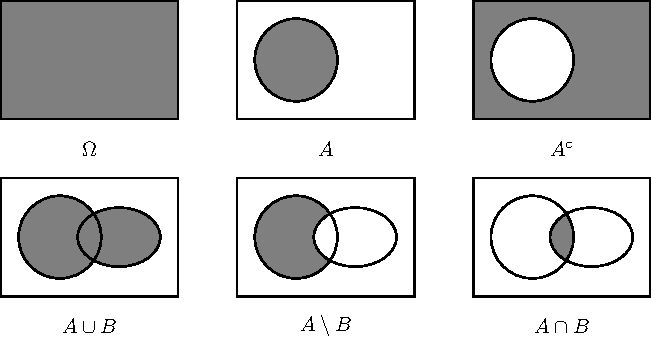
\includegraphics{figures/tikz/venn.pdf}
		\captionof{figure}{Venn图}
		\label{fig:venn}
	\end{center}
\end{definition}

\begin{theorem}
	{de Morgan定律}{de Morgan's laws}
	对于事件集$\{A_i\}_{i\in I}$,其中指标集$I$可以是有限集或无限集,有恒等式:
	\[
		\kh{\bigcup\nolimits_{i\in I} A_i}\c = \bigcap\nolimits_{i\in I} A_i\c.
	\]
\end{theorem}

\paragraph{概率的解释}古典解释,等可能性,Bertrand悖论;频率解释,主观解释。

\section{公理化定义}

概率函数$\P$应给出事件(及其运算)的概率。因此,$\P$作为一个映射的定义域(称为事件空间$\cF$)除了应包括样本空间$\Omega$和其若干子集外,还应满足事件运算的封闭性。

\begin{definition}
	{幂集}{power set}
	定义$\Omega$的幂集(power set)为$\Omega$所有子集构成的集合,记作$2^\Omega$。
\end{definition}

\begin{definition}{$\sigma$-代数}{sigma-algebra}
	幂集的子集$\Sigma\subset 2^\Omega$若满足事件运算的封闭性:
	\begin{compactenum}
		\item $\Omega \in \Sigma;$
		\item $\forall A \in \Sigma, A\c \in \Sigma;$
		\item 特别地,若$\forall A_i \in \Sigma$,则
		$\bigcup\nolimits_{i\in I} A_i \in \Sigma.$
	\end{compactenum}
	则称$\Sigma$是$\Omega$的$\sigma$-代数($\sigma$-algebra)。
\end{definition}

借助测度论的语言,我们要求事件空间$\cF$必须是样本空间$\Omega$的一个$\sigma$-代数。

\begin{example}{$\sigma$-代数}{sigma-algebra}
	若$\Omega=\{a,b,c,d\}$,则一个平凡的$\sigma$-代数
	\[
		\Sigma_1=\{\varnothing, \Omega\},
	\]
	另一个$\sigma$-代数可以为
	\[
		\Sigma_2=\{\varnothing,\{a\},\{b,c,d\},\{b\},\{a,c,d\},\{a,b\},\{c,d\},\Omega\}.
	\]
\end{example}
\begin{definition}{概率}{probability}
	定义概率(probability)~$\P:\cF\to\RR$,满足:
	\begin{compactenum}
		\item $\forall A\in\cF,\P(A)\geqslant 0;$
		\item $\P (\Omega)=1;$
		\item (\textbf{加法公理})~$\forall A_i \in \cF,A_iA_j=\varnothing(i\neq j),$
		\begin{equation}
			\P\kh{\bigcup\nolimits_{i\in I} A_i}=\sum\nolimits_{i\in I}\P(A_i).
		\end{equation}
	\end{compactenum}
	称$(\Omega,\cF,\P)$构成了概率空间(probability space)。
\end{definition}
\begin{corollary}
	由定义,可推出:
	\begin{compactenum}
		\item $\forall A\in\cF,\P(A)\leqslant 1;$
		\item $\P(\varnothing)=0;$
		\item 
		% 若$A_i$两两互斥,即$\forall A_i \in \cF,A_iA_j=\varnothing\,(i\neq j)$,则
		% \[
		% 	\P\kh{\bigcup_{i=1}^n A_i}=\sum_{i=1}^n\P(A_i)
		% \]
		特别地,$\P(A)+\P(A\c)=1;$
		\item $\forall A\subset B,\P(A)\leqslant\P(B);$
		\item $\P(A+B)=\P(A)+\P(B)-\P(AB).$推广之,得到
	\end{compactenum}
\end{corollary}
\begin{theorem}{容斥恒等式}{inclusion and exclusion identities}
	容斥恒等式(inclusion and exclusion identities)
	\begin{align}\notag
		\P\kh{\bigcup_{i=1}^nA_i}&=\sum_{i=1}^n\P(A_i)-\sum_{i<j}^n\P(A_i\cap A_j)+\cdots+\P\kh{\bigcap_{i=1}^nA_i}\\
		&=\sum_{r=1}^n(-)^{r+1}\sum_{i_1<\cdots<i_r}\P\kh{\bigcap_{k=1}^rA_{i_k}}.
	\end{align}
\end{theorem}
\begin{example}{乱序}{derangement}
	$n$个人每人一个帽子,混在一起随机分配,求无人拿到自己帽子的概率。

	记$A_i=$第$i$个人拿到自己的帽子,则
	\[
		\P(A_i)=\frac1n\equiv\frac{(n-1)!}{n!}.
	\]
	至少一个人拿到自己的帽子:
	\begin{align*}
		\P\kh{\bigcup_{i=1}^nA_i}&=\sum_{r=1}^n(-)^{r+1}\sum_{i_1<\cdots<i_r}\P\kh{\bigcap_{k=1}^rA_{i_k}}\\
		&=\sum_{r=1}^n(-)^{r+1}\binom nr\frac{(n-r)!}{n!}=\sum_{r=1}^n(-)^{r+1}\frac1{r!}\\
		&=1-\frac1{2!}+\frac1{3!}+\cdots+(-)^{n+1}\frac1{n!}.
	\end{align*}
	故所求概率即
	\[
		\P\kh{\bigcap_{i=1}^nA_i\c}=1-1+\frac1{2!}-\frac1{3!}+\cdots+(-)^n\frac1{n!}\to\frac1{\e{}}.
	\]
	\tcblower
	这个问题称为乱序(derangement)问题,乱序数(subfactorial)记作
	\begin{equation}
		\label{eq:subfactorial}
		!n=n!\biggkh{1-1+\frac1{2!}-\frac1{3!}+\cdots+(-)^n\frac1{n!}}=\biggfkh{\frac{n!}e}=\floor{\frac{n!}e+1/2}.
	\end{equation}
	其中$[x]$表示最接近$x$的整数,$\floor x$表示向下取整。前几个乱序数见 \href{https://oeis.org/A000166}{OEIS.A000166}
	\[
		!0=1,\quad !1=0,\quad !2=1,\quad !3=2,\quad !4=9,\quad !5=44,\quad !6=265.%\quad !7=1854,\quad !8=14833,\quad !9=133496.
	\]	
\end{example}

\section{条件概率}

\begin{definition}{条件概率}{conditional probability}
	给定$B$事件发生的条件下,$A$事件发生的条件概率(conditional probability)为
	\begin{equation}
		\P(A|B):=\frac{\P(A\cap B)}{\P(B)}
	\end{equation}
	其中$\P(B)>0.$
\end{definition}

\begin{remark}
	条件概率可用于缩小样本空间。
\end{remark}

\begin{corollary}
	% 事实上,给定$B$且$\P(B)>0$,则
	$\P(\cdot|B):\cF\to\RR$是概率函数,$\bigkh{\Omega,\cF,\P(\cdot|B)}$也是概率空间。
\end{corollary}

\begin{theorem}{乘法法则}{multiplication rule}
	由条件概率的定义可以直接导出:
	\begin{equation}
		\P(A\cap B)=\P(B)\P(A|B)=\P(A)\P(B|A).
	\end{equation}
	一般推广:
	\[
		\P(A_1\cap\cdots\cap A_n)=\P(A_1)\P(A_2|A_1)\cdots\P(A_n|A_1\cap\cdots\cap A_{n-1}).
	\]
\end{theorem}

\begin{remark}
	加上限制条件以后,算概率可能会变简单。
\end{remark}

\begin{remark}
	已观测到$A$事件$\iff\P(A|A)\equiv 1$,绝非$\P(A)=1$。
\end{remark}

\section{独立事件}

\begin{definition}{独立事件}{independent event}
	定义$A,B$相互独立(independent)当
	\begin{equation}
		\P(A\cap B)=\P(A)\P(B).
	\end{equation}
\end{definition}

$B$事件发生与否,不影响$A$事件发生的概率:
\[
	\P(A|B)=\P(A)\iff\frac{\P(A\cap B)}{\P(B)}=\frac{\P(A\cap\Omega)}{\P(\Omega)}.
\]

\begin{corollary}
	$A,B$独立$\iff A\c,B$独立$\iff A,B\c$独立$\iff A\c,B\c$独立。
\end{corollary}

\begin{definition}{多个事件的独立}{}
	$A,B,C$相互独立等价于:
	\begin{compactenum}
		\item $A,B,C$两两独立;
		\item $\P(A\cap B\cap C)=\P(A)\P(B)\P(C)$
	\end{compactenum}
	进而定义可数个事件$A_1,A_2,\ldots$相互独立:任取有限个事件$A_{i_1},\ldots,A_{i_n}$都有
	\[
		\P(A_{i_1}\cap\cdots\cap A_{i_n})=\P(A_{i_1})\cdots\P(A_{i_n}).
	\]
\end{definition}

\begin{remark}
	在三个事件相互独立的定义中,两个条件都是必要的,只知其一不可推出另一个条件。
\end{remark}


\begin{definition}{条件独立}{conditional independent}
	若
	\[
		\P(A\cap B|E)=\P(A|E)\P(B|E),
	\]
	则$A,B$关于事件$E$条件独立(conditional independent)。
\end{definition}

\begin{remark}
	$A,B$关于$E$条件独立$\xcancel{\iff}A,B$独立。(既不充分也不必要)
\end{remark}

\section{Bayes公式}

\begin{definition}
	{分割}{partition}
	事件空间的子集$\{B_i\}_{i\in I}\subset\cF$若满足:
	\begin{compactenum}
		\item $\bigcap\nolimits_{i\in I} B_i=\Omega;$
		\item $\forall i\neq j,\enspace B_iB_j=\varnothing;$
		\item $\forall i,\enspace\P(B_i)>0.$
	\end{compactenum}
	则称$\{B_i\}_{i\in I}$是样本空间$\Omega$的一个分割。
\end{definition}

\begin{theorem}{全概率公式}{total probability formula}
	给定样本空间$\Omega$的一个分割$\{B_i\}_{i\in I}$,则$A$事件的概率
	\begin{equation}
		\P(A)=\sum_{i\in I}\P(B_i)\P(A|B_i)
	\end{equation}
\end{theorem}
\begin{example}{假阳性悖论}{false positive paradox}
	假设有一种疾病,10000人中约有一人发病,患病者检测出阳性(真阳性)的概率为99\%,未患病者检测出阳性(假阳性)的概率为0.1\%。求检测出阳性的人患病的概率。

	$B=$患病,$A=$阳性,题中对应的概率为
	\[
		\P(B)=10^{-4},\enspace
		\P(A|B)=0.99,\enspace
		\P(A|B\c)=10^{-3},
	\]
	故检测出阳性的人患病的概率为
	\[
		\P(B|A)=\frac{\P(AB)}{\P(A)}=\frac{\P(B)\P(A|B)}{\P(B)\P(A|B)+\P(B\c)\P(A|B\c)}\doteq 9\%
	\]
	并不高。其原因在于:发病率$\P(B)<$假阳性的概率$\P(A|B\c)$。

	如何避免假阳性悖论?可以进行二次检测,使得
	$\P(B)>\P(AA|B\c)=10^{-6}$
	
\end{example}
\begin{example}{赌徒}{gambler}
	两个人赌博。假设甲的本金为$i$元,乙的本金为$n-i$。甲赢的概率为$p$,乙赢的概率为$q=1-p$。
	每赌一局输家给赢家1元,其中一人输光则游戏结束。求甲成为最终赢家的概率$Q_i$。

	$A=$甲最终赢,$B=$甲本局赢,由全概率公式
	\[
		\P(A)=\P(B)\P(A|B)+\P(B\c)\P(A|B\c).
	\]
	即
	\[
		Q_i=pQ_{i+1}+qQ_{i-1},%\implies p(Q_{i+1}-Q_i)=(1-p)(Q_i-Q_{i-1}).
	\]
	且有边界条件:$Q_0=0,Q_n=1$,
	\[
		Q_i=\begin{cases}
			\frac in,&p=q=1/2\\[2ex]
			\frac{1-(q/p)^i}{1-(q/p)^n},&p\neq 1/2
		\end{cases}
	\]
	取$n=6,i=1,2,\ldots,n-1$,绘制不同概率下的$Q_i$分布图:
	\begin{center}
		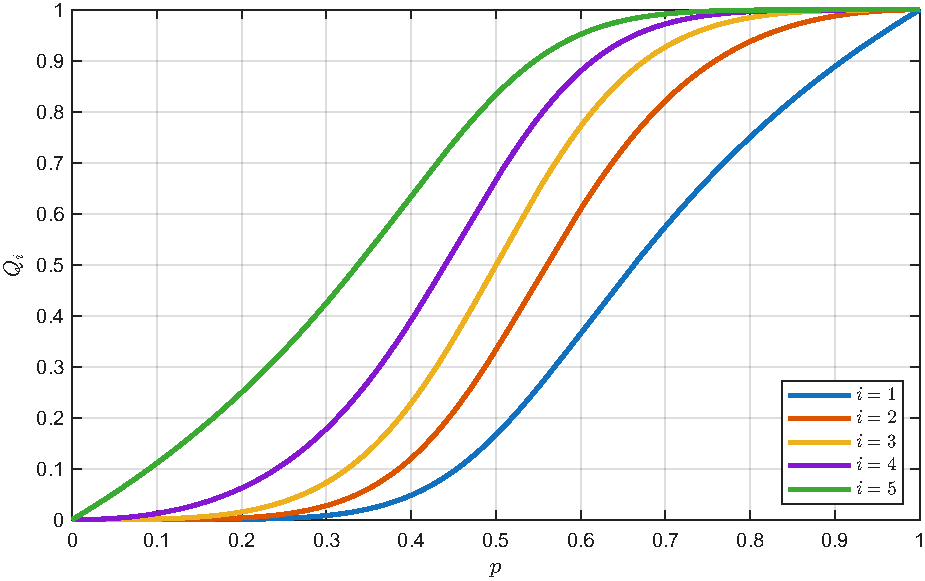
\includegraphics[width=0.7\linewidth]{figures/gamble.pdf}
		\captionof{figure}{赌徒问题的概率分布图}
	\end{center}
\end{example}

\begin{theorem}{Beyas公式}{Beyas formula}
	Beyas公式即
	\begin{equation}
		\P(B_i|A)=\frac{\P(B_i)\P(A|B_i)}{\P(A)}=\frac{\P(B_i)\P(A|B_i)}{\sum_{j\in I}\P(B_j)\P(A|B_j)}
	\end{equation}
	称$\P(B_i)$为\textbf{先验概率}(priori probability),$\P(B_i|A)$为\textbf{后验概率}(posterior probability)。
\end{theorem}

% \begin{remark}
% 	这个公式的重要性不仅在数学意义上,还在于先验概率$\P(B_i)$ v.s.后验概率$\P(B_i|A)$
% \end{remark}

\begin{remark}
	计算正确的概率、正确计算概率、正确使用概率。
\end{remark}
